% =====================================================================
%  ch01b.tex ------ 第 1 章 §1.2 仿射 Lie 代数的表示 + §1.3 Wess--Zumino--Witten 模型
%  原书 p.11--p.24（PDF 31--44）
% =====================================================================

% [原文 p.11]
\section{仿射 Lie 代数的表示}

\takeaway{本节先备齐 $\fsl_2(\C)$ 的表示论（最高权表示、Verma 模、Clebsch--Gordan 规则），再构造仿射 Lie 代数 $\hat{\fg}$ 的 level $k$ 最高权模 $\mathcal{H}_{k,\lambda}$，并用 Sugawara 算子把它实现为 Virasoro 代数的表示，中心荷为 $3k/(k+2)$。}

一般地，复 Lie 代数 $\fg$ 的线性表示，是指一个线性映射 $\rho:\fg\to\End(V)$：其中 $V$ 是复线性空间，$\End(V)$ 是 $V$ 的线性变换全体，且 $\rho$ 满足
\[
  \rho([X,Y])=\rho(X)\rho(Y)-\rho(Y)\rho(X).
\]
这时称 $V$ 为左 $\fg$ 模，或简称 $\fg$ 模。此外，对 $X\in\fg$、$v\in V$，也常把 $\rho(X)v$ 简记为 $Xv$。

本节把仿射 Lie 代数 $\hat{\fg}$ 的表示论中本书所需的程度汇总起来。细节请参阅文献 [8] 等。这里只就 $\fg=\fsl_2(\C)$ 的情形说明。此时 $\hat{\fg}$ 称为 $A_1^{(1)}$ 型仿射 Lie 代数。

首先复习 $\fg=\fsl_2(\C)$ 的表示论。$\fsl_2(\C)$ 是迹为 $0$ 的 $2$ 行 $2$ 列复矩阵全体，以
\[
  [X,Y]=XY-YX,\qquad X,Y\in\fsl_2(\C)
\]
赋予 Lie 代数结构。作为复线性空间，$\fsl_2(\C)$ 是 $3$ 维的，
\[
  H=\begin{pmatrix}1&0\\0&-1\end{pmatrix},\qquad
  E=\begin{pmatrix}0&1\\0&0\end{pmatrix},\qquad
  F=\begin{pmatrix}0&0\\1&0\end{pmatrix}
\]
构成它的基。这些基元满足交换关系
\[
  [H,E]=2E,\qquad [H,F]=-2F,\qquad [E,F]=H.
\]

对 $X,Y\in\fg$ 令 $\langle X,Y\rangle=\Tr(XY)$，则 $\fg$ 上由此确定一个非退化的对称双线性形式。它就是 $\fg$ 的 Cartan--Killing 型。对上面的生成元 $H,E,F$，有 $\langle H,H\rangle=2$，$\langle E,F\rangle=1$，$\langle H,E\rangle=0$，$\langle H,F\rangle=0$。

取关于 Cartan--Killing 型的正规正交基 $\{I_\mu\}$，用
\[
  C=\sum_\mu I_\mu I_\mu
\]
定义 $\fg$ 的泛包络代数 $U(\fg)$ 中的元素 $C$。称 $C$ 为 Lie 代数 $\fg$ 的 Casimir 元。Casimir 元也可表为
\[
  C=\frac{1}{2}H^2+EF+FE,
\]
并且可以验证：对一切 $X\in U(\fg)$ 都成立 $[C,X]=0$。

% [Tutor Note: 这里取 $\langle X,Y\rangle=\Tr(XY)$，于是 $\langle H,H\rangle=2$、$\langle E,F\rangle=1$。正是这组归一化使 $\{I_\mu\}$ 正规正交下的 $C=\sum_\mu I_\mu I_\mu$ 等于 $\frac12H^2+EF+FE$；下一段算出 Casimir 的特征值为 $2j(j+1)$，而 §1.2 末共形权公式里出现的 $j(j+1)$ 恰是它的一半，两处不要混。]

% [原文 p.12]
设 $\lambda$ 为复数。取 $\fg=\fsl_2(\C)$，说左 $\fg$ 模 $V$ 是最高权 $\lambda$ 的最高权表示（highest weight representation），是指下列条件 (1)、(2) 成立。
\begin{enumerate}[label=(\arabic*),leftmargin=2.2em,itemsep=2pt]
  \item $V$ 中存在非零向量 $v$，使 $Hv=\lambda v$、$Ev=0$。
  \item $V$ 作为复线性空间由 $F^nv\ (n=0,1,\dots)$ 生成。
\end{enumerate}
条件 (1) 中的向量 $v$ 称为最高权向量（highest weight vector）。又，若条件 (2) 中 $F^nv\ (n=0,1,\dots)$ 全部线性无关，则称 $V$ 为最高权 $\lambda$ 的 Verma 模（Verma module），记作 $M_\lambda$。注意：这里把 $\lambda$ 取作复数，而对一般的 Lie 代数，最高权要作为 Cartan 子代数的对偶空间的元素来表述。

$\lambda$ 取一般复数时，Verma 模 $M_\lambda$ 是不可约 $\fg$ 模；但对特殊的 $\lambda$，可以把 $M_\lambda$ 对极大子模作商，得到 $\fg$ 的不可约表示。取 $\lambda$ 为 $0$ 以上的整数，令 $\lambda=2j$。设 $V_\lambda$ 是以 $u_m\ (m=j,j-1,\dots,-j+1,-j)$ 为基的 $\lambda+1$ 维复向量空间，并用
\begin{align*}
  Hu_m&=2mu_m,\\
  Eu_m&=\sqrt{(j+m+1)(j-m)}\;u_{m+1},\\
  Fu_m&=\sqrt{(j+m)(j-m+1)}\;u_{m-1}
\end{align*}
定义 Lie 代数 $\fg$ 在 $V_\lambda$ 上的作用。此时 $u_j$ 是最高权向量。又，$F^{\lambda+1}u_j=0$，故 $V_\lambda$ 可表为 Verma 模的商模，是 $\lambda+1$ 维的不可约表示。也称 $V_\lambda$ 为 $\fsl_2(\C)$ 的自旋 $j$ 的不可约表示。Casimir 元 $C$ 属于 $U(\fg)$ 的中心，故在每个不可约表示 $V_\lambda$ 上作用为标量。计算它在最高权向量上的作用可知，该标量为 $2j(j+1)$。已知 $\fsl_2(\C)$ 的有限维不可约表示，都与上面这样构造出的某个表示同构。

% [原文 p.13]
对 $V_\lambda$ 的对偶空间 $V_\lambda^*=\Hom_\C(V_\lambda,\C)$，可以把 $\fg$ 在 $V_\lambda^*$ 上从右的作用唯一地定成满足
\[
  \langle\xi X,\eta\rangle=\langle\xi,X\eta\rangle,\qquad
  \xi\in V_\lambda^*,\ \eta\in V_\lambda,\ X\in\fg
\]
的作用。其中 $\langle\ ,\ \rangle$ 是 $V_\lambda^*$ 与 $V_\lambda$ 的自然配对。这样得到的右 $\fg$ 模 $V_\lambda^*$，称为 $\fg$ 的最高权 $\lambda$ 的右不可约表示。若用 $\{u_m^*\}$ 表示基 $\{u_m\}$ 的对偶基，则对此右作用有 $u_m^*H=2mu_m$，$u_j^*F=0$，而 $V_\lambda^*$ 由 $u_j^*E^n\ (n=0,1,\dots,\lambda)$ 张成。

% [Tutor Note: 原书 p.13 作 $u_m^*H=2mu_m$，右端漏了对偶基的星号，与同一句里「对偶基」的设定不符，疑为笔误；按配对 $\langle u_m^*,Hu_n\rangle=\langle u_m^*,2nu_n\rangle=2m\delta_{mn}$ 应为 $u_m^*H=2mu_m^*$。]

此外，用这个右作用，把 $\fg$ 在 $V_\lambda^*$ 上的作用 $\rho^*$ 定为 $\rho^*(X)\xi=-\xi X$（$X\in\fg$，$\xi\in V_\lambda^*$），则
\[
  \rho^*([X,Y])=\rho^*(X)\rho^*(Y)-\rho^*(Y)\rho^*(X),
\]
从而 $V_\lambda^*$ 具有左 $\fg$ 模的结构。称之为原表示 $V_\lambda$ 的双对表示（dual representation）。这里讨论的是 $\fg=\fsl_2(\C)$ 的情形，此时 $V_\lambda$ 与其双对表示 $V_\lambda^*$ 作为左 $\fg$ 模同构。

一般地，对 Lie 代数 $\fg$ 的表示 $V,W$，把 $\fg$ 在 $V\otimes W$ 上的作用定为
\[
  X(v\otimes w)=Xv\otimes w+v\otimes Xw,\qquad
  X\in\fg,\ v\in V,\ w\in W,
\]
称之为表示的张量积（tensor product）。$\fg=\fsl_2(\C)$ 时，关于张量积分解为不可约表示，下述命题即著名的 Clebsch--Gordan 规则。

\begin{proposition}{1.4}
（Clebsch--Gordan 规则）对 $\fg=\fsl_2(\C)$ 的不可约表示的张量积，
\[
  \Hom_{\fsl_2(\C)}(V_{\lambda_1}\otimes V_{\lambda_2}\otimes V_{\lambda_3},\C)\cong\C
\]
成立的充要条件是
\[
  \lambda_1+\lambda_2+\lambda_3\in 2\Z,\qquad
  |\lambda_1-\lambda_2|\le\lambda_3\le\lambda_1+\lambda_2
\]
成立。上述条件不满足时，$\Hom_{\fsl_2(\C)}(V_{\lambda_1}\otimes V_{\lambda_2}\otimes V_{\lambda_3},\C)=0$。
\end{proposition}

特别地，关于 $V=V_1$ 的张量积分解为不可约成分，有
\[
  V\otimes V=V_0\oplus V_2,\qquad
  V\otimes V\otimes V=2V_1\oplus V_3,
\]

% [原文 p.14]
\[
  V\otimes V\otimes V\otimes V=2V_0\oplus 3V_2\oplus V_4
\]
等等。表示空间前的数字表示该表示的重复度，一般可用二项式系数表出。

% [Tutor Note: 这里 $V_\lambda$ 的维数是 $\lambda+1=2j+1$，同一段里 $\lambda$ 与 $j$ 两套记法并存（$\lambda=2j$）。命题 1.4 的条件 $\lambda_1+\lambda_2+\lambda_3\in2\Z$ 换回自旋就是 $j_1+j_2+j_3\in\Z$；此后凡见 $\lambda$ 都指最高权，勿与自旋 $j$ 或维数 $\lambda+1$ 混用。]

下面谈仿射 Lie 代数的表示。对 Laurent 级数 $f(t)\in\C((t))$，把能表成 $f(t)=\sum_{n>0}a_nt^n$ 的全体记为 $A_+$，把能表成 $f(t)=\sum_{n<0}a_nt^n$ 的全体记为 $A_-$。仿射 Lie 代数 $\hat{\fg}$ 的子 Lie 代数 $\mathcal{N}_+,\mathcal{N}_0,\mathcal{N}_-$ 分别定义为
\[
  \mathcal{N}_+=[\fg\otimes A_+]\oplus\C E,\qquad
  \mathcal{N}_0=\C H\oplus\C c,\qquad
  \mathcal{N}_-=[\fg\otimes A_-]\oplus\C F,
\]
则有 Lie 代数的直和分解
\[
  \hat{\fg}=\mathcal{N}_+\oplus\mathcal{N}_0\oplus\mathcal{N}_-.
\]

设 $k,\lambda$ 为复数。$\hat{\fg}$ 模 $\hat{V}_{k,\lambda}$ 称为 $\hat{\fg}$ 的 level $k$、最高权 $\lambda$ 的表示，是指下列条件 (1)、(2) 成立。
\begin{enumerate}[label=(\arabic*),leftmargin=2.2em,itemsep=2pt]
  \item $\hat{V}_{k,\lambda}$ 中存在非零向量 $v$，使 $\mathcal{N}_+v=0$、$cv=kv$、$Hv=\lambda v$。
  \item 记 $U(\mathcal{N}_-)$ 为 $\mathcal{N}_-$ 的泛包络代数，则 $\hat{V}_{k,\lambda}=U(\mathcal{N}_-)v$。
\end{enumerate}
利用条件 (1)、(2) 以及 $c$ 属于 $\hat{\fg}$ 的中心，可知对一切 $u\in\hat{V}_{k,\lambda}$ 都有 $cu=ku$。条件 (1) 中出现的 $v$ 称为 $\hat{V}_{k,\lambda}$ 的最高权向量。$\hat{V}_{k,\lambda}$ 由形如
\[
  a_1\cdots a_rv,\qquad a_1,\dots,a_r\in\mathcal{N}_-,\ r\ge 0
\]
的元素生成。

$\hat{\fg}$ 的 level $k$、最高权 $\lambda$ 的表示中，在 $U(\mathcal{N}_-)$ 上以 $v$ 为生成元的秩 $1$ 自由模，称为 Verma 模，记作 $M_{k,\lambda}$。$\hat{\fg}$ 的 level $k$、最高权 $\lambda$ 的表示 $\hat{V}_{k,\lambda}$，一般可表为 $M_{k,\lambda}$ 的商模：即可取 $M_{k,\lambda}$ 的子模 $N$，把 $\hat{V}_{k,\lambda}$ 写成 $\hat{V}_{k,\lambda}=M_{k,\lambda}/N$。特别地，取 $N$ 为极大子模，就得到 $\hat{\fg}$ 的不可约表示作为商模。对一般的参数 $k,\lambda$，Verma 模 $M_{k,\lambda}$ 本身不可约；但对特殊的 $k,\lambda$，已知 Verma 模实际上可约。

% [Tutor Note: $A_+$ 的定义取 $n>0$（不含常数项），$A_-$ 取 $n<0$，故常数项 $\fg\otimes1$ 不属于 $\mathcal{N}_\pm$；$\mathcal{N}_0=\C H\oplus\C c$ 只补上零次的两个方向。正因如此，零次元 $X\otimes t^0$ 与 $H,c$ 是分开处理的，下面 (1.9)、(1.10) 才要按 $n=0$ 与 $n\ne0$ 分两种写法。]

% [原文 p.15]
$k$ 为正整数时，Kac 给出了下述结果。

\begin{proposition}{1.5}
$k$ 为正整数，$\lambda$ 为满足 $0\le\lambda\le k$ 的整数。则 $\chi=(E\otimes t^{-1})^{k-\lambda+1}v$ 满足 $\mathcal{N}_+\chi=0$，且 $U(\mathcal{N}_-)\chi$ 是 $M_{k,\lambda}$ 的极大子模。商模
\[
  \mathcal{H}_{k,\lambda}=M_{k,\lambda}/U(\mathcal{N}_-)\chi
\]
是 $\hat{\fg}$ 的不可约表示。这里 $v$ 是上面说明过的 Verma 模的生成元。
\end{proposition}

这样便构造出了 level $k$、最高权 $\lambda$ 的不可约表示。这种表示称为 integrable highest weight module。关于命题 1.5 的证明，请参阅文献 [8] 等。满足上述条件的 $\lambda$，称为 level $k$ 的最高权。又，$\chi$ 称为零向量（null vector）。$\mathcal{H}_{k,\lambda}$ 以 $\fsl_2(\C)$ 的有限维不可约表示 $V_\lambda$ 为子空间。在 level $k$ 已明确固定的情形下，也把 $\mathcal{H}_{k,\lambda}$ 简记为 $\mathcal{H}_\lambda$。

又，关于 $\mathcal{H}_\lambda$ 的对偶空间 $\mathcal{H}_\lambda^*$，可以把右 $\hat{\fg}$ 模的结构唯一地定成如下形式：关于自然配对，
\[
  \langle\xi\alpha,\eta\rangle=\langle\xi,\alpha\eta\rangle,\qquad
  \xi\in\mathcal{H}_\lambda^*,\ \eta\in\mathcal{H}_\lambda,\ \alpha\in\hat{\fg}.
\]
关于这个右作用，$\mathcal{H}_\lambda^*$ 中存在作为右 $U(\mathcal{N}_+)$ 模的生成元 $v^*$，且满足 $v^*\mathcal{N}_-=0$。

又，用这个右作用，把 $\hat{\fg}$ 在 $\mathcal{H}_\lambda^*$ 上的作用 $\rho^*$ 定为 $\rho^*(X\otimes t^n)\xi=-\xi X\otimes t^{-n}$（$X\in\fg$，$\xi\in\mathcal{H}_\lambda^*$），则 $\mathcal{H}_\lambda^*$ 具有左 $\hat{\fg}$ 模的结构。称之为 $\mathcal{H}_\lambda$ 的双对表示（dual representation）。

下面说明 Virasoro 代数在 $\mathcal{H}_\lambda$ 上的作用。$\Diff^+(S^1)$ 作为映射 $f:S^1\to G$ 的参数化取换，作用在环路群 $LG$ 上。仿射 Lie 代数由环路群 Lie 代数的形式版本即环路代数作中心扩张而得，因此自然期望：在它的表示空间上，有 $S^1$ 上多项式向量场构成的 Lie 代数的中心扩张，即 Virasoro 代数作用。实际上已知有下述所谓 Sugawara 算子（Sugawara operator），它是 Casimir 元的无限维推广，用它便可定义 Virasoro 代数

% [原文 p.16]
在 $\mathcal{H}_{k,\lambda}$ 上的作用。

具体地说，取 $\{I_\mu\}$ 为关于 Cartan--Killing 型的 $\fg$ 的基，$n\ne0$ 时令
\begin{equation}
  L_n=\frac{1}{2(k+2)}\sum_{j\in\Z}\sum_\mu I_\mu\otimes t^{-j}\cdot I_\mu\otimes t^{n+j} \tag{1.9}
\end{equation}
$n=0$ 时令
\begin{equation}
  L_0=\frac{1}{k+2}\sum_{j\ge 1}\sum_\mu I_\mu\otimes t^{-j}\cdot I_\mu\otimes t^{j}+\frac{1}{2(k+2)}\sum_\mu I_\mu\cdot I_\mu \tag{1.10}
\end{equation}
以此作为形式定义。上述 $n\ne0$ 的情形有 $I_\mu\otimes t^{-j}\cdot I_\mu\otimes t^{n+j}=I_\mu\otimes t^{n+j}\cdot I_\mu\otimes t^{-j}$。又，$L_n$ 的定义式含无限和，但要注意：对 level $k$ 的最高权表示 $\mathcal{H}_{k,\lambda}$ 的元素 $v$，$L_nv$ 总可表为有限和。对基 $I_\mu\ (\mu=1,2,3)$ 计算 $[L_m,I_\mu\otimes t^n]$，便可证明下述命题。

% [Tutor Note: (1.10) 中 $j$ 只跑 $j\ge1$，等于把 (1.9) 里 $j$ 与 $-j$ 成对的两项合并后只取一半，所以前因子从 $1$ 变成 $1/(k+2)$；若照 (1.9) 用 $j\in\Z$ 又保留 $1/(k+2)$，$L_0$ 会多算一倍。]

\begin{proposition}{1.6}
对整数 $m,n$，作为 $\hat{\fg}$ 在表示空间 $\mathcal{H}_{k,\lambda}$ 上的作用，有交换关系
\[
  [L_m,X\otimes t^n]=-nX\otimes t^{m+n},\qquad X\in\fg .
\]
\end{proposition}

再用命题 1.6 计算，可得下述命题。

\begin{proposition}{1.7}
作为 Sugawara 算子 $L_m\ (m\in\Z)$ 在 $\mathcal{H}_{k,\lambda}$ 上的作用，有交换关系
\[
  [L_m,L_n]=(m-n)L_{m+n}+\frac{m^3-m}{12}\,\delta_{m+n,0}\,\frac{3k}{k+2}.
\]
也就是说，Sugawara 算子使 $\mathcal{H}_{k,\lambda}$ 成为 Virasoro 代数的表示空间，$c$ 的作用为乘以 $3k/(k+2)$。
\end{proposition}

% [Tutor Note: 这里把 Virasoro 交换关系写成 $[L_m,L_n]=(m-n)L_{m+n}+\frac{m^3-m}{12}\delta_{m+n,0}c$，其中 $c=3k/(k+2)$。$k\to\infty$ 时 $c\to3$，正是 $\fg=\fsl_2(\C)$ 的维数。$\delta_{m+n,0}$ 说明中心项只在 $n=-m$ 时出现，而 $m^3-m$ 在 $m=0,\pm1$ 处为零，故子代数 $\{L_{-1},L_0,L_1\}$ 上中心项不起作用。]

按算子 $L_0$ 的特征值，$\mathcal{H}_\lambda=\mathcal{H}_{k,\lambda}$ 可作如下分解。先看 $L_0$ 在 $V_\lambda$ 上的作用：对 $u\in V_\lambda$ 有
\[
  L_0u=\frac{1}{2(k+2)}\Bigl(\sum_\mu I_\mu\cdot I_\mu\Bigr)u=\frac{j(j+1)}{k+2}\,u,
\]
其中已令 $\lambda=2j$。把这个特征值 $j(j+1)/(k+2)$ 记为 $\Delta_\lambda$，称为共形权

% [原文 p.17]
（conformal weight）。用命题 1.6 可知，$L_0$ 在 $\mathcal{H}_\lambda$ 中的特征值可写成 $\Delta_\lambda+d$，其中 $d$ 为 $0$ 以上的整数。把属于特征值 $\Delta_\lambda+d$ 的特征空间记为 $\mathcal{H}_{\lambda,d}$，则有直和分解
\begin{equation}
  \mathcal{H}_\lambda=\bigoplus_{d\ge0}\mathcal{H}_{\lambda,d}. \tag{1.11}
\end{equation}
这里每个 $\mathcal{H}_{\lambda,d}$ 都是有限维的，特别地 $\mathcal{H}_{\lambda,0}=V_\lambda$。

\section{Wess--Zumino--Witten 模型}

\takeaway{WZW 作用 $S_\Sigma(f)$ 由能量项与 Wess--Zumino 项组成，其指数 $\exp(-S_\Sigma(f))$ 不依赖三维延拓 $B$ 与扩张 $\tilde f$ 的取法。据此可在环路群 $LG_\C$ 上造出复线丛 $\mathcal{L}$（及其双对丛），其纤维元素给出 $LG_\C$ 的中心扩张，并承载规范群 $\Map(\Sigma,G_\C)$ 的左右作用。}

设 $\Sigma$ 为无边界的紧 Riemann 面。取 Lie 群 $G=SU(2)$，设 $f:\Sigma\to G$ 为光滑映射。

如 §1.1 所述，对 $SU(2)$ 的元素 $X$，Maurer--Cartan 形式 $\theta=X^{-1}dX$ 是取值于 Lie 代数 $\fsu(2)$、定义在 $SU(2)$ 上的一次微分形式，且关于 $SU(2)$ 的左作用不变。又，三次微分形式
\[
  \sigma=\frac{1}{24\pi^2}\Tr(\theta\wedge\theta\wedge\theta)
\]
是 $SU(2)$ 的左不变体积元，其 de Rham 上同调类给出 $H^3(SU(2),\Z)$ 的生成元。

对光滑映射 $f:\Sigma\to G$，积分
\[
  E_\Sigma(f)=-\sqrt{-1}\int_\Sigma\Tr(f^{-1}\partial f\wedge f^{-1}\bar\partial f)
\]
称为映射 $f$ 的能量（energy）。以下固定一个称为 level（层次）的整数 $k$。用映射 $f$ 的能量，把 Wess--Zumino--Witten 作用 $S_\Sigma(f)$ 定义为
\[
  S_\Sigma(f)=\frac{k}{4\pi}E_\Sigma(f)
  -\frac{\sqrt{-1}k}{12\pi}\int_B\Tr\bigl(\tilde f^{-1}d\tilde f\wedge\tilde f^{-1}d\tilde f\wedge\tilde f^{-1}d\tilde f\bigr).
\]
这里 $B$ 是以 $\Sigma$ 为边界的定向紧三维流形，$\tilde f:B\to G$ 是 $f$ 作为光滑映射的扩张。

% [Tutor Note: $\sigma$ 前的 $1/24\pi^2$ 是归一化因子，使 $\int_{SU(2)}\sigma=1$ 恰为 $H^3(SU(2),\Z)$ 的生成元；正因如此，WZW 项前面的 $\sqrt{-1}k/12\pi$ 才保证 $\exp(-S_\Sigma(f))$ 单值，$k$ 必须是整数。若把 $\sigma$ 的常数改成 $1/8\pi^2$（另一种常见约定），$k$ 的整性条件随之改变。]

% [原文 p.18]
又，$\tilde f^{-1}d\tilde f$ 表示 Maurer--Cartan 形式 $X^{-1}dX$ 经 $\tilde f$ 的拉回。

\begin{lemma*}{1.8}
对 Wess--Zumino--Witten 作用 $S_\Sigma(f)$，
\[
  \exp(-S_\Sigma(f))
\]
不依赖于上述 $B$ 以及映射扩张 $\tilde f$ 的取法，只由 Riemann 面 $\Sigma$ 与映射 $f:\Sigma\to G$ 决定。
\end{lemma*}

\begin{proof}
再取一个以 $\Sigma$ 为边界的定向紧三维流形，记为 $B'$。又设 $\tilde f':\Sigma\to G$ 是 $f$ 作为光滑映射到 $B'$ 的扩张。把流形 $B'$ 的定向反转所得记为 $-B'$，把 $B$ 与 $B'$ 沿边界 $\Sigma$ 粘合，所得的无边界定向紧三维流形记为 $M$。为考察 Wess--Zumino--Witten 作用的变化，注意积分
\[
  \frac{k}{24\pi^2}\Bigl(\int_B\Tr(\tilde f^{-1}d\tilde f\wedge\tilde f^{-1}d\tilde f\wedge\tilde f^{-1}d\tilde f)
  -\int_{B'}\Tr(\tilde f'^{-1}d\tilde f'\wedge\tilde f'^{-1}d\tilde f'\wedge\tilde f'^{-1}d\tilde f')\Bigr).
\]
定义映射 $F:M\to G$，使其在 $B$ 与 $B'$ 上的限制分别为上述 $\tilde f$ 与 $\tilde f'$。这个积分用三次微分形式 $\sigma$ 可表为
\[
  k\int_M F^*\sigma .
\]
由于 $\sigma$ 给出 $H^3(G,\Z)$ 的生成元，积分值为整数。因此 $\exp(-S_\Sigma(f))$ 不依赖 $B$ 与映射扩张 $\tilde f$ 的取法，这就证明了所要的结论。
\end{proof}

% [Tutor Note: 原书 p.18 把第二个扩张写成 $\tilde f':\Sigma\to G$，但同一句又称它是 $f$ 到 $B'$ 的扩张，定义域应为 $B'$；疑为笔误。证明的关键一步是「积分值必为整数」，即 $\sigma$ 的 de Rham 类属于整系数上同调，故 $\exp(-2\pi\sqrt{-1}\cdot\text{整数})=1$。]

Wess--Zumino--Witten 作用 $S_\Sigma(f)$ 中出现的
\[
  \frac{\sqrt{-1}k}{12\pi}\int_B\Tr(\tilde f^{-1}d\tilde f\wedge\tilde f^{-1}d\tilde f\wedge\tilde f^{-1}d\tilde f)
\]
称为 Wess--Zumino 项。后面将详细说明：在能量项上加上这个 Wess--Zumino 项，便可构造出关于 Riemann 面的局部共形变换不变的场论。为此起重要作用的，是下述 Polyakov--Wiegmann 等式。

\begin{proposition*}{1.9}
（Polyakov--Wiegmann 等式）对 Riemann 面 $\Sigma$ 到 Lie 群 $G$ 的两个光滑映射 $f,g$，其积 $fg:\Sigma\to G$ 由 $(fg)(z)=f(z)g(z)$（$z\in\Sigma$）定义。
\end{proposition*}

% [原文 p.19]
这时
\[
  \exp(-S_\Sigma(fg))=\exp\Bigl(-S_\Sigma(f)-S_\Sigma(g)
  -\frac{\sqrt{-1}k}{2\pi}\int_\Sigma\Tr(f^{-1}\bar\partial f\wedge\partial gg^{-1})\Bigr)
\]
成立。

\begin{proof}
证明由简单计算完成，故只述梗概。首先注意：一般地，对取值于矩阵的 $p$ 次微分形式 $\omega$ 与 $q$ 次微分形式 $\eta$，取迹有
\[
  \Tr(\omega\wedge\eta)=(-1)^{pq}\Tr(\eta\wedge\omega).
\]
用这一等式计算
\[
  I=\int_\Sigma\Tr\bigl((fg)^{-1}\partial(fg)\wedge(fg)^{-1}\bar\partial(fg)\bigr),
\]
并利用
\begin{align*}
  I_1&=\int_\Sigma\Tr\bigl(f^{-1}\partial f\wedge f^{-1}\bar\partial f
    +g^{-1}\partial g\wedge g^{-1}\bar\partial g\bigr),\\
  I_2&=\int_\Sigma\Tr\bigl(f^{-1}\partial f\wedge\bar\partial gg^{-1}
    +\partial gg^{-1}\wedge f^{-1}\bar\partial f\bigr),
\end{align*}
则 $I=I_1+I_2$。进一步，对 Wess--Zumino 项用 $df^{-1}=-f^{-1}dff^{-1}$ 与 Stokes 定理，即得所要结论。
\end{proof}

% [Tutor Note: 这一步的关键是 $I_2$ 的两个交叉项与 Wess--Zumino 项改写后的贡献合成一个全微分，故只剩 $I_1$。另请注意等式第三项只含 $f$ 的反全纯导数 $\bar\partial f$ 与 $g$ 的全纯导数 $\partial g$：当 $f$ 全纯或 $g$ 反正则时该项为零，这正是本节末命题 1.11 的出发点。]

以下采用下述记号
\[
  \Gamma_\Sigma(f,g)=-\frac{\sqrt{-1}k}{2\pi}\Bigl(\int_\Sigma\Tr(f^{-1}\bar\partial f\wedge\partial gg^{-1})\Bigr).
\]

对 Lie 群 $G=SU(2)$ 的复化 $G_\C=SL(2,\C)$，考虑从单位圆板
\[
  D=\{z\in\C\mid |z|\le1\}
\]
出发的光滑映射 $f_0:D\to G_\C$。用 $D_\infty$ 表示 Riemann 球面 $\CP^1=\C\cup\{\infty\}$ 中 $D$ 的补集的闭包，即
\[
  D_\infty=\{z\in\C\mid |z|\ge1\}\cup\{\infty\}.
\]
把 $f_0:D\to G_\C$ 作为光滑映射延拓到整个 Riemann 球面 $\CP^1$，记之为 $f$。用 $f_\infty$ 表示 $f:\CP^1\to G_\C$ 在 $D_\infty$ 上的限制。对这个 $f$，与前面同样地

% [原文 p.20]
\[
  \exp(-S_{\CP^1}(f))\in\C
\]
便确定下来。下面考察这个量随 $f_0$ 延拓到 $\CP^1$ 的方式如何变化。

再取一个 $f_0:D\to G_\C$ 作为光滑映射到整个 $\CP^1$ 的延拓，记为 $f':\CP^1\to G_\C$。$f'$ 可用光滑映射 $h:\CP^1\to G_\C$ 写成 $f'=fh$。这里对 $z\in D$ 有 $h(z)=e$，其中 $e$ 表示 Lie 群 $G_\C$ 的单位元。用 $h_\infty$ 表示映射 $h$ 在 $D_\infty$ 上的限制。由 Polyakov--Wiegmann 等式，
\[
  \exp(-S_{\CP^1}(fh))=\exp\bigl(-S_{\CP^1}(f)-S_{\CP^1}(h)+\Gamma_{\CP^1}(f,h)\bigr)
\]
成立。又，由于对 $z\in D$ 有 $h(z)=e$，
\[
  \Gamma_{\CP^1}(f,h)=\Gamma_{D_\infty}(f_\infty,h_\infty).
\]
因此得到等式
\begin{equation}
  \exp(-S_{\CP^1}(fh))=\exp\bigl(-S_{\CP^1}(f)-S_{\CP^1}(h)+\Gamma_{D_\infty}(f_\infty,h_\infty)\bigr) \tag{1.12}
\end{equation}

下面用上面的考察说明：把 $\exp(-S_D(f_0))$ 看作环路群 $LG_\C$ 上某个复线丛的纤维的元素来定义，是自然的。用 $\Map_0(D_\infty,G_\C)$ 表示满足 $\varphi(\infty)=e$ 的光滑映射 $\varphi:D_\infty\to G_\C$ 的全体。用极坐标把 $\frac{1}{z}=re^{\sqrt{-1}\theta}$ 表出，令 $\varphi(z)=p_r(e^{\sqrt{-1}\theta})$，则
\[
  p_r:S^1\longrightarrow G_\C,\qquad 0\le r\le1
\]
对每个固定的 $r$ 给出 $G_\C$ 的一个环路。特别地，$r=0$ 时得到把 $S^1$ 的所有点映到 $G_\C$ 单位元的常值环路。因此 $p_r\ (0\le r\le1)$ 是环路群 $LG_\C$ 中的光滑道路，而 $p_0$ 是环路群的单位元。由此可见，$\Map_0(D_\infty,G_\C)$ 可与以环路群 $LG_\C$ 的单位元为起点的光滑道路全体等同。

在直积
\[
  \Map_0(D_\infty,G_\C)\times\C
\]
上引入下述等价关系 $\sim$。对 $\Map_0(D_\infty,G_\C)\times\C$ 的两个元素 $(f_\infty,u)$、$(g_\infty,v)$，规定
\[
  (f_\infty,u)\sim(g_\infty,v)
\]

% [原文 p.21]
是指下列条件 (1)、(2) 成立。
\begin{enumerate}[label=(\arabic*),leftmargin=2.2em,itemsep=3pt]
  \item $f_\infty(z)=g_\infty(z)$，$z\in\partial D$。
  \item 写成 $g_\infty=f_\infty h_\infty$ 时，
  \[
    v=u\exp\bigl(-S_{\CP^1}(h)+\Gamma_{D_\infty}(f_\infty,h_\infty)\bigr)
  \]
  成立。其中 $h:\CP^1\to G_\C$ 是把 $h_\infty:D_\infty\to G_\C$ 作为在 $D$ 上恒取单位元 $e$ 的恒等映射延拓到整个 $\CP^1$ 而得者。
\end{enumerate}

把上述等价关系 $\sim$ 下的等价类全体 $\Map_0(D_\infty,G_\C)\times\C/\sim$ 记为 $\mathcal{L}$。用嵌入映射 $\iota:\partial D\to D$，把投影 $\pi:\mathcal{L}\to LG_\C$ 定为 $\pi([f_\infty,u])=f_\infty\circ\iota$。这里 $[f_\infty,u]$ 表示 $(f_\infty,u)$ 所属的等价类。由此投影可知，$\mathcal{L}$ 具有环路群 $LG_\C$ 上的复线丛结构。如上所述，若把 $\Map_0(D_\infty,G_\C)$ 与以环路群 $LG_\C$ 单位元为起点的光滑道路全体等同，则条件 (1) 是说道路的端点重合，条件 (2) 则是关于和乐的条件。这与 §1.1 中复线丛的构造类似。实际上可以证明，作为复线丛，$\mathcal{L}$ 与 §1.1 中 $LG_\C$ 上的基本复线丛 $L$ 的 $k$ 次张量幂 $L^{\otimes k}$ 同构。下述引理成立。

% [Tutor Note: 条件 (1) 只保证两条道路端点相同，能否拼成纤维上的同一元素要看条件 (2)；条件 (2) 右端正是把 $\exp(-S_{\CP^1}(h))$ 与和乐因子 $\Gamma_{D_\infty}$ 相比较，故说它是关于和乐的条件。$\mathcal{L}\cong L^{\otimes k}$ 说明此处的 $k$ 与 WZW 作用里的 level 是同一个整数。]

\begin{lemma*}{1.10}
$\exp(-S_D(f_0))$ 作为复线丛 $\mathcal{L}$ 在 $f_0\circ\iota$ 上的纤维的元素确定下来。
\end{lemma*}

\begin{proof}
再取一个 $f_0:D\to G_\C$ 作为光滑映射到整个 $\CP^1$ 的延拓，记为 $f':\CP^1\to G_\C$，并把它写成 $f'=fh$。只需证明
\[
  (f_\infty,\exp(-S_{\CP^1}(f)))\sim(f_\infty h_\infty,\exp(-S_{\CP^1}(fh)))
\]
即可，而这由等式 (1.12) 立得。于是断言得证。
\end{proof}

接着构造 $\mathcal{L}$ 的双对丛 $\mathcal{L}^{-1}$。先用 $\Map_0(D,G_\C)$ 表示满足 $\varphi(0)=e$ 的光滑映射 $\varphi:D\to G_\C$ 的全体。在 $\Map_0(D,G_\C)\times\C$ 上如下定义等价关系 $\sim$。对 $\Map_0(D,G_\C)\times\C$ 的元素 $(f_0,u)$、$(g_0,v)$，规定
\[
  (f_0,u)\sim(g_0,v)
\]

% [原文 p.22]
是指下列条件 (1)、(2) 成立。
\begin{enumerate}[label=(\arabic*),leftmargin=2.2em,itemsep=3pt]
  \item $f_0(z)=g_0(z)$，$z\in\partial D$。
  \item 写成 $g_0=f_0h_0$ 时，
  \[
    v=u\exp\bigl(-S_{\CP^1}(h)+\Gamma_D(f_0,h_0)\bigr)
  \]
  成立。
\end{enumerate}

此时 $\mathcal{L}^{-1}=\Map_0(D,G_\C)\times\C/\sim$ 在投影 $\pi([f_0,u])=f_0\circ\iota$ 之下具有环路群 $LG_\C$ 上的复线丛结构。进一步，与引理 1.10 的讨论同样地，对 $f_\infty:D_\infty\to G_\C$，
\[
  \exp(-S_{D_\infty}(f_\infty))=[f_0,\exp(-S_{\CP^1}(f))]
\]
作为复线丛 $\mathcal{L}^{-1}$ 在 $f_\infty\circ\iota$ 上的纤维的元素确定下来。

复线丛 $\mathcal{L},\mathcal{L}^{-1}$ 的配对如下给出。令 $f_0\circ\iota=f_\infty\circ\iota=\gamma$，把配对
\[
  \mathcal{L}\times\mathcal{L}^{-1}\longrightarrow\C
\]
定义为 $([f_\infty,u],[f_0,v])=uv\exp(S_{\CP^1}(f))$。再次用等式 (1.12) 可证右端不依赖等价类代表元的取法。又，关于这个配对，
\[
  \bigl\langle\exp(-S_D(f_0)),\exp(-S_{D_\infty}(f_\infty))\bigr\rangle=\exp(-S_{\CP^1}(f))
\]
成立，这也容易直接验证。

% [Tutor Note: 配对定义的指数是正的 $\exp(S_{\CP^1}(f))$，与 $\exp(-S_\Sigma(f))$ 的负号相反：双对丛 $\mathcal{L}^{-1}$ 的作用正是把这个正号吃回去。也正因如此，(1.13) 的积里出现的是 $-\Gamma_D$ 而不是 $+\Gamma_D$。]

这里构造的复线丛 $\pi:\mathcal{L}\to LG_\C$ 与环路群 $LG_\C$ 的中心扩张的关系，说明如下。把满足 $s(\gamma)=0\in\mathcal{L}_\gamma$ 的映射 $s:LG_\C\to\mathcal{L}$ 称为零截面，用 $\widehat{LG}_\C$ 表示从复线丛 $\mathcal{L}$ 去掉零截面的像 $s(LG_\C)$ 后所得的集合。对从单位圆板 $D$ 到 $G_\C$ 的光滑映射 $g$，用边界的参数化 $\iota:\partial D\to D$，令 $\gamma=g\circ\iota$，则由上面的构造可定义
\[
  \exp(-S_D(g))\in\mathcal{L}_\gamma .
\]
又，复线丛 $\mathcal{L}$ 的纤维的任意点，都可用适当的 $g:D\to G_\C$ 表为 $z\exp(-S_D(g))\ (z\in\C)$ 的形状。对 $g_i:D\to G_\C\ (i=1,2)$，令 $\gamma_i=g_i\circ\iota$，对 $\exp(-S_D(g_i))\in\mathcal{L}_{\gamma_i}$，把它们的积定义为
\begin{equation}
  \exp(-S_D(g_1))\bullet\exp(-S_D(g_2))=\exp(-S_D(g_1g_2)-\Gamma_D(g_1,g_2)) \tag{1.13}
\end{equation}

% [原文 p.23]
把它作为复线性映射扩张，便定出积
\[
  \mathcal{L}_{\gamma_1}\times\mathcal{L}_{\gamma_2}\longrightarrow\mathcal{L}_{\gamma_1\gamma_2},
\]
并可在 $\widehat{LG}_\C$ 上引入积结构。此定义不依赖 $g_1,g_2$ 的取法，且由此积可确认 $\widehat{LG}_\C$ 具有群的结构。进一步，把对 $D$ 的所有元素都对应 $G_\C$ 单位元的映射记为 $e:D\to G_\C$，由 $i(z)=z\exp(-S_D(e))$ 定义 $i:\C^*\to\widehat{LG}_\C$，便得到群的正合列
\[
  1\longrightarrow\C^*\xrightarrow{\ i\ }\widehat{LG}_\C\xrightarrow{\ \pi\ }LG_\C\longrightarrow1 .
\]
这给出环路群 $LG_\C$ 的中心扩张。

设 $\Sigma$ 为边界同胚于若干个 $S^1$ 的并集的紧 Riemann 面。设 $\Sigma$ 上给定复结构。固定边界的参数化 $p_i:S^1\to\partial\Sigma\ (1\le i\le m)$。有 $\partial\Sigma=\bigcup_{i=1}^m p_i(S^1)$，并设边界上的定向由 Riemann 面 $\Sigma$ 的定向诱导。如图 1.1 所示，把单位圆板 $D_i\ (1\le i\le m)$ 的边界分别粘到 $\Sigma$ 的边界 $p_i(S^1)$ 上，所得的无边界紧 Riemann 面记为 $\tilde\Sigma$。

\begin{figure}[htbp]
  \centering
  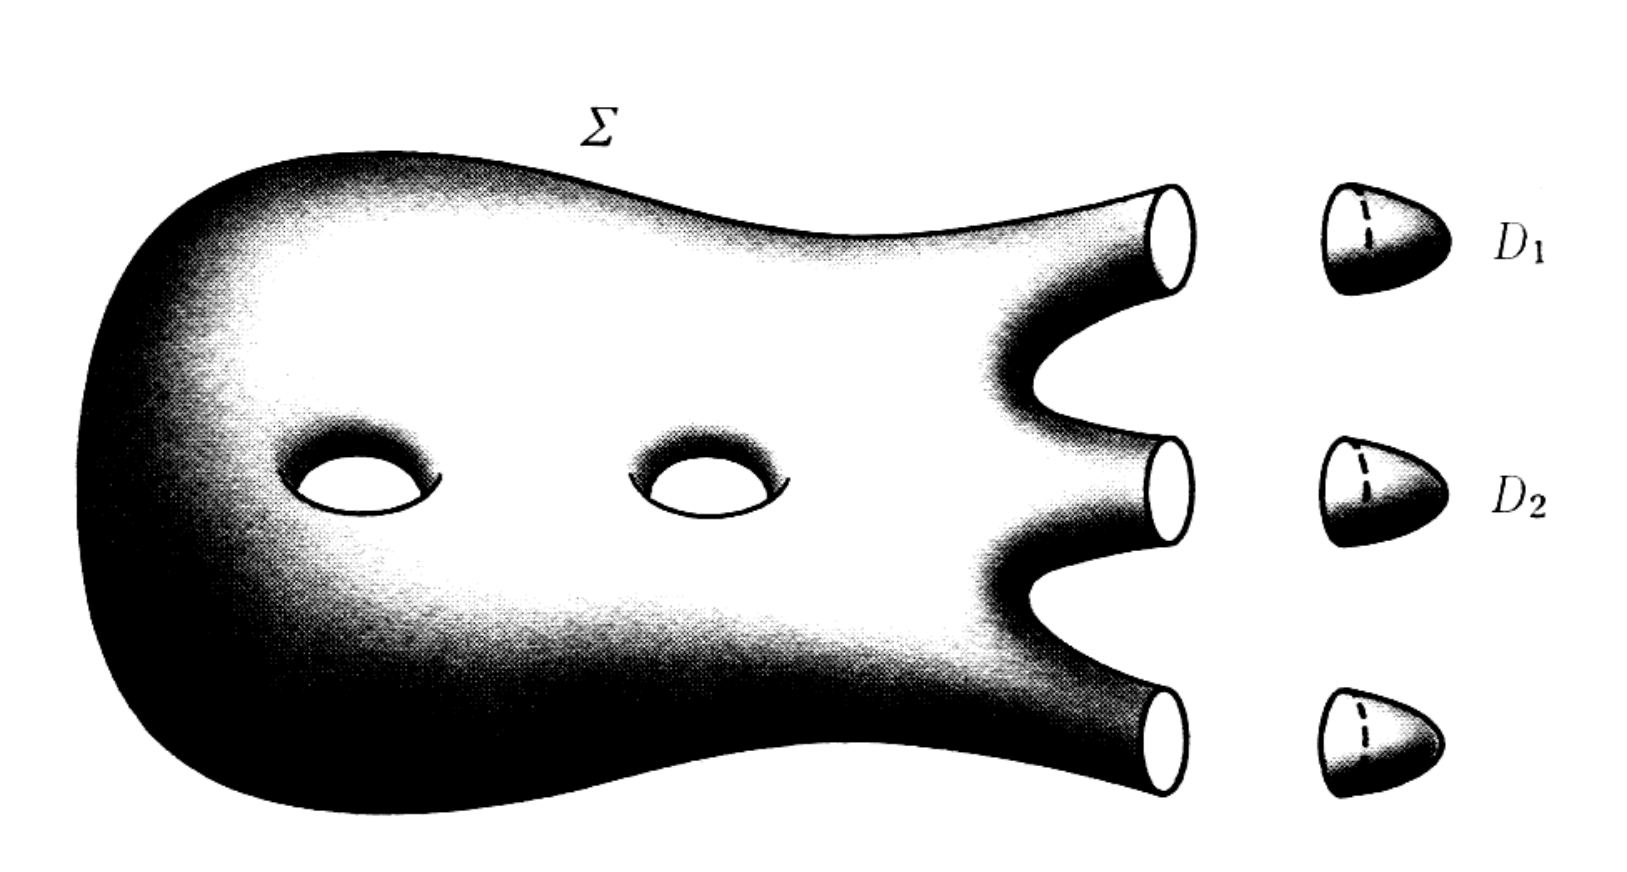
\includegraphics[width=0.70\textwidth]{figures/fig1.1.png}
  \figtitle{1.1}{把圆板 $D_1,D_2,\dots$ 粘到 $\Sigma$ 的边界上（原书 p.23）}
\end{figure}

对光滑映射 $g:\Sigma\to G_\C$，来定义 $\exp(-S_\Sigma(g))$。把 $g$ 作为光滑映射延拓到 $\tilde\Sigma$，记为 $\tilde g:\tilde\Sigma\to G_\C$。又用 $g_i$ 表示 $\tilde g$ 在 $D_i$ 上的限制。对每个单位圆板 $D_i$ 应用上面关于 $D_\infty$ 的复线丛 $\mathcal{L}^{-1}$ 的构造，$\exp(-S_{D_i}(g_i))$ 便作为纤维 $\mathcal{L}^{-1}_{g\circ p_i}$ 的元素确定下来。用它把 $\exp(-S_\Sigma(g))$

% [原文 p.24]
定义为满足
\[
  \Bigl\langle\exp(-S_\Sigma(g)),\bigotimes_{i=1}^m\exp(-S_{D_i}(g_i))\Bigr\rangle=\exp(-S_{\tilde\Sigma}(\tilde g))
\]
的 $\bigotimes_{i=1}^m\mathcal{L}_{g\circ p_i}$ 的元素。这里同样用 Polyakov--Wiegmann 等式可以确认：它不依赖 $g$ 的扩张 $\tilde g$ 的取法，只由 $g$ 与 $\Sigma$ 决定。

这样，对光滑映射 $g:\Sigma\to G_\C$，$\exp(-S_\Sigma(g))$ 便作为复线丛 $\mathcal{L}$ 的纤维的张量积 $\bigotimes_{i=1}^m\mathcal{L}_{g\circ p_i}$ 的元素定义出来了。以下为简便起见，只处理 $m=1$ 的情形。用 $p:S^1\to\partial\Sigma$ 表示边界的参数化。对光滑映射 $f:\Sigma\to G_\C$，用式 (1.13) 定义的积，把 $f$ 在 $\mathcal{L}$ 上的左作用 $l(f)$ 定为
\[
  l(f)\exp(-S_\Sigma(g))=\exp(-S_\Sigma(f))\bullet\exp(-S_\Sigma(g)).
\]
这里由 Polyakov--Wiegmann 等式可知
\begin{equation}
  \exp(-S_\Sigma(f))\bullet\exp(-S_\Sigma(g))=\exp(-S_\Sigma(fg)-\Gamma_\Sigma(f,g)) \tag{1.14}
\end{equation}
成立。同样地，把 $f$ 在 $\mathcal{L}$ 上的右作用 $r(f)$ 定为
\[
  r(f)\exp(-S_\Sigma(g))=\exp(-S_\Sigma(g))\bullet\exp(-S_\Sigma(f)).
\]
用 $\Map(\Sigma,G_\C)$ 表示光滑映射 $f:\Sigma\to G_\C$ 的全体。这是 $\Sigma$ 上平凡 $G_\C$ 丛的规范群（gauge group）。由到边界的限制
\[
  p^*:\Map(\Sigma,G_\C)\longrightarrow LG_\C,
\]
规范群 $\Map(\Sigma,G_\C)$ 从左右两侧作用在环路群 $LG_\C$ 上。进一步可知，由上述左作用与右作用，规范群 $\Map(\Sigma,G_\C)$ 在 $LG_\C$ 上的作用可提升为复线丛 $\mathcal{L}$ 上的作用。

对全纯映射 $h:\Sigma\to G_\C$ 决定的左作用 $l(h)$，以及对反全纯映射 $\bar h$ 决定的右作用 $r(\bar h)$，在下述意义下表现出协变性。

\begin{proposition*}{1.11}
对全纯映射 $h:\Sigma\to G_\C$，
\[
  l(h)\exp(-S_\Sigma(g))=\exp(-S_\Sigma(hg))
\]
成立。又，对反全纯映射 $\bar h:\Sigma\to G_\C$，
\[
  r(\bar h)\exp(-S_\Sigma(g))=\exp(-S_\Sigma(g\bar h))
\]
成立。
\end{proposition*}

% --- 命题 1.11 的证明起于 p.24 末行、续于 p.25 开头；为保证 proof 环境完整，本块已译至 p.25 的 ■ 处（ch01c 从 p.25「Wess--Zumino--Witten 模型本来の目的は…」接续，勿重复）---
\begin{proof}
对全纯映射 $h$，由 $\bar\partial h=0$ 可知
\[
  \Gamma_\Sigma(h,g)=-\frac{\sqrt{-1}k}{2\pi}\Bigl(\int_\Sigma\Tr(h^{-1}\bar\partial h\wedge\partial gg^{-1})\Bigr)=0
\]
成立。再结合 (1.14) 形式的 Polyakov--Wiegmann 等式，即得所要结果。对反全纯映射 $\bar h$ 的右作用，同样用 $\partial\bar h=0$ 可证。
\end{proof}
% --- 跨块补完结束 ---

% [Tutor Note: 证明只用了一条：$\Gamma_\Sigma(h,g)$ 的被积式含 $h^{-1}\bar\partial h$，$h$ 全纯时整个为零，于是 (1.14) 退化为 $\exp(-S_\Sigma(hg))$。反全纯的 $\bar h$ 恰好使 $\partial$ 一侧消失。故左作用只对全纯 $h$、右作用只对反全纯 $\bar h$ 协变，一般的 $h$ 只会剩下带 $\Gamma$ 的因子。]

% 块尾跨页句：命题 1.11 的证明起于 p.24 末行、续于 p.25 开头，本块已译至 p.25 的「同様に示される。」（■）；tr03 自「これと，(1.14) の形の Polyakov--Wiegmann の等式をあわせて」一句起接续，勿重复。

% CHUNK ch01b DONE

